\documentclass{standalone}
\usepackage{tikz}
\usetikzlibrary{positioning}
\usetikzlibrary{calc}
\usetikzlibrary{decorations.markings,arrows}
\pdfpagewidth=100mm
\pdfpageheight=100mm
\begin{document}
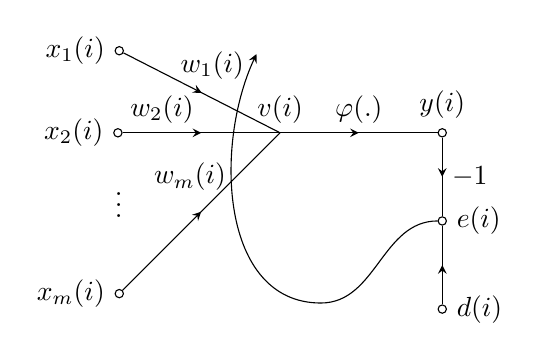
\begin{tikzpicture}[
    middlearrow/.style n args={4}{
        decoration={
            markings,
            mark=at position 0.5 with {\arrow{stealth}, \path ++(#3,#4) node[#1] {#2};}
          },
        postaction={decorate}
      },
  ]

  \coordinate[label=above:{ $v(i)$}] (V1) at (0, 0) {};
  \node [circle,draw=black, fill=white, inner sep=0pt,minimum size=3pt, label=left:{ $x_1(i)$}, above left=1cm and 2cm of V1] (X1)  {};
  \node [circle,draw=black, fill=white, inner sep=0pt,minimum size=3pt, label=left:{ $x_2(i)$}, left= 2cm of V1] (X2)  {};
  \coordinate[label={  $\vdots$}, below left=1.2cm and 2.05cm of V1] (VDOTS) {};
  \node [circle,draw=black, fill=white, inner sep=0pt,minimum size=3pt, label=left:{ $x_m(i)$}, below left=2cm and 2cm of V1] (XM) {};
  \node [circle,draw=black, fill=white, inner sep=0pt,minimum size=3pt, label=above:{ $y(i)$}, right= 2cm of V1] (YI) {};
  \node [circle,draw=black, fill=white, inner sep=0pt,minimum size=3pt, label=right:{ $e(i)$}, below= 1cm of YI] (EI) {};
  \node [circle,draw=black, fill=white, inner sep=0pt,minimum size=3pt, label=right:{ $d(i)$}, below= 1cm of EI] (DI) {};
  \coordinate[below left=1cm and 1.5cm of EI] (INTERMEDIATE) {};
  \coordinate[above left=1cm and 0.3cm of V1] (FINAL) {};

  \draw [ middlearrow={above}{ $w_1(i)$}{0.1}{0.1}] (X1) -- (V1);
  \draw [ middlearrow={above}{ $w_2(i)$}{-0.5}{0}] (X2) -- (V1);
  \draw [ middlearrow={above}{ $w_m(i)$}{0}{0.2}] (XM) -- (V1);
  \draw [ middlearrow={above}{ $\varphi (.)$}{0}{0}] (V1) -- (YI);
  \draw [ middlearrow={right}{ $-1$}{0}{0}] (YI) -- (EI);
  \draw [ middlearrow={right}{}{0}{0}] (DI) -- (EI);
  \draw [] (EI) to[out=180,in=0] (INTERMEDIATE);
  \draw [-stealth] (INTERMEDIATE) to[out=180,in=245] (FINAL);

\end{tikzpicture}
\end{document}


